\documentclass[final]{anthology-ch}

\usepackage{booktabs}
\usepackage{graphicx}

\title{Why Do Older Books Survive (Sometimes)? Modelling the Time Distribution of Manuscripts with a Birth-Death Approach}

\author[1]{Ulysse Godreau}[
orcid=0000-0001-9799-2410
]

\author[1]{Théo Moins}[
orcid=0009-0002-7191-5761
]

\author[1]{Kelly Christensen}[
orcid=0000-0002-7236-874X
]

\author[1]{Jean-Baptiste Camps}[
orcid=0000-0003-0385-7037
]

\affiliation{1}{École nationale des Chartes, Université PSL, Paris, France}

\keywords{Cultural Transmission, Evolutionary Modelling, Birth-Death Process, Philology, Medieval Manuscripts}

\pubyear{2025}
\pubvolume{3}
\pagestart{1508}
\pageend{1518}
\conferencename{Computational Humanities Research 2025}
\conferenceeditors{Taylor Arnold, Margherita Fantoli, and Ruben Ros}
\doi{10.63744/c4L67UxjQVI3}
\paperorder{95}

\addbibresource{bibliography.bib}

\newcommand{\nbar}{\overline{n}}
\newcommand{\Nbar}{\overline{N}}
\newcommand{\rmd}{\mathrm{d}}

\begin{document}

\maketitle

\begin{abstract}
Understanding the survival of ancient manuscripts dating back to different periods and centuries is crucial for gathering insights into historical textual traditions and, more generally, cultural history.
Previous studies have modelled the transmission of texts, particularly in manuscript form, as a birth-death process, in which the existing manuscript witnesses of a given text are simultaneously being copied and destroyed at given rates.
However, these models have not fully accounted for key  properties observed in real historical written traditions, such as the temporal distribution of surviving manuscripts and the heavy-tailed distribution of surviving witnesses by text.
In this study, we refine the birth-death process to better explain these dynamics. We investigate the role of extrinsic historical factors on the transmission of texts, through the use of variable copy and destruction rates to reflect extrinsic historical factors, such as fluctuations in the book market or disruptions like wars. Additionally, we look into the effect of intrinsic features of the book themselves and the uses for which they were designed, be it to be stored on a library shelf or to be intensively used and copied.
We test those refinements against empirical data collected for medieval traditions. Preliminary results indicate that these enhancements allow us to establish variations in production and destruction rates that align with known macro-level historical dynamics. This revised approach helps explain why we do in fact preserve (some) of the older manuscripts, and not only their most recent descendants, offering a more comprehensive understanding of manuscript survival.
\end{abstract}

\section{Introduction}

Early scholars, since at least the late 18\textsuperscript{th} century, seem to have intuitively understood the transmission of texts in manuscript form has a type of evolutionary process, based on descent with innovation, that can be represented as an evolutionary tree~\cite{bengel_apparatus_1763,schlyter_corpus_1827}. From an original, copies are made and circulated, giving rise in time to new copies. Modifications are induced to the text during the copy process, that can then be inherited by a given copy's descendants. Yet, it is not until the late 20\textsuperscript{th} century than it has been explicitly modelled as a stochastic Birth-Death (BD) process, that can be simulated with computers or understood analytically~\cite{weitzman_computer_1982,weitzman_evolution_1987}. If these researches have showcased the underlying role of chance and of extrinsic factors (historical contingencies) in the transmission and survival of texts and manuscripts, and have proved the ability of a simple BD process to approximate many relevant features of historical textual traditions, a recent study has demonstrated that the BD process still fails to account for some of the typical properties observed empirically in historical textual traditions~\cite{camps2025transmissiontextswrittencultures}.
Three main mismatches can indeed be identified between the result of a Birth-Death process, and observed historical data. They relate to:
\begin{enumerate}
\item the distribution of witnesses per text, that in historical data follows a heavy-tail, Pareto-like behaviour, instead of an exponential distribution. This means that, in historical data, there often exist a small number of texts with a very high number of witnesses;
\item the distribution of witnesses (and texts) in time, that display, in historical data, fluctuations that cannot be approximated by a constant rate model;
\item the topological properties of trees, in particular related to the so-called `bifidity' (the presence of a root outdegree of 2, i.e. of two main branches), a known feature of textual traditions since Bédier~\cite{bedier_tradition_1928}, and more generally their structural imbalance between branches, that in historical stemmata collections tend to be even higher than the already high level in simulations resulting from a BD process.
\end{enumerate}

These mismatches point to inadequacies in the BD model, and hint at the presence of some dynamics that are not captured by this simple null-model. One obvious reason might be that, for the sake of generality and simplicity, the BD model used by Camps et al.~\cite{camps2025transmissiontextswrittencultures} used rates of copy and destruction of manuscripts that remained constant both in time --~neutralising the effect that extrinsic historical factors have on book production and preservation~-- and between manuscripts --~neutralising the differences between different types of manuscripts that we know exist.
In contrast to them, earlier work by Weitzman~\cite{weitzman_evolution_1987} did try to implement variations in time of the copy and destruction rates, based on historical expertise and observed time distribution of surviving manuscripts, according to their putative dating.
Yet, as will be shown below, variation of these rates is probably not enough to fully account for the way in which older manuscripts may in some cases constitute a quite important part of the preserved witnesses of a given text.

Indeed, in this research, we make the hypothesis that two features, taken in combination, can provide a better account of the aforementioned properties of historical textual traditions, and help mitigate the main mismatches observed with a result of a constant rate BD process.

The first one is the variation in time of the copy and destruction rates, to reflect historical contingencies, such as changes in fashion, book production techniques or events such as wars, plagues or economic crises, that may impact book production. These variations can actually be fitted on the basis of historical data, using analytic methods.

The second is the existence of different types of books, that may possess different copy or destruction probabilities. In particular, we investigate the effect of a system with two different types: on one hand, books dedicated to preservation, such as the so-called ``\textit{manuscrits de librairie}'' (or ``\textit{de bibliothèque}''), i.e. books ordered from workshops by collectors and intended either for silent reading or for private performance~\cite{tyssens_tradition_1988}, that can often be richly ornamented. On the other hand, books dedicated to more practical uses. This second type can characterise a book such as an exemplar involved in the production of new books, via for instance the quire-based \textit{pecia} copy system, where medieval students would rent, quire by quire, the textbooks they needed to copy for themselves~\cite{weichselbaumer2015quod}, or simply plain books, often in small format, whose main value was the text they contained, such as the \textit{libelli} (``booklets'')~\cite{hanna_booklets_1986}
or the so-called ``\textit{manuscrits de jongleur}'', though this terminology is a bit misleading~\cite{tyssens_tradition_1988}.

On the basis of these two refinements, we test our hypothesis by confronting the updated BD process with empirical data collected for Medieval traditions in French.

\section{Improvement to the Birth-Death process}

\subsection{Modelling the apparition of texts}

The simplest model emulating the elementary features of manuscript transmission that we consider is the Birth-Death (BD) process. In this setting, manuscript witnesses are represented by independent agents associated with two states: living --~that is, available for reproduction~-- and dead, meaning lost or destroyed. During an elementary time step $\mathrm{d}t$, each living witness in the population may undergo two processes:
\begin{itemize}
\item
With probability $\lambda\mathrm{d}t$, the manuscript is copied and gives birth to a new living manuscript. We call $\lambda$ the \emph{birth rate} of the process, standing for the copy rate of manuscripts;
\item
With probability $\mu\mathrm{d}t$, the manuscript dies and becomes inactive, with $\mu$ the \emph{death rate} of the process, that is the destruction rate of manuscripts.
\end{itemize}
We furthermore model the apparition of original manuscripts of new texts by allowing new independent manuscripts to be created at rate $\Lambda$. The rates $\lambda, \mu$ are assumed to be the same for all agents. Keeping track of the genealogical relations between manuscripts, the population at any time can be represented by a forest of tree-shaped graphs where a manuscript/node $i$ is connected to a node $j$ by a directed edge $(i,j)$ if $j$ was copied from $i$. Each tree in the forest then represents the full manuscript tradition of a given text, whose root is the original and the surviving manuscripts at the end of the simulation the witnesses of this text (See \autoref{fig:bd_dynamics}, for a simple example).

\begin{figure}[htbp]
\centering
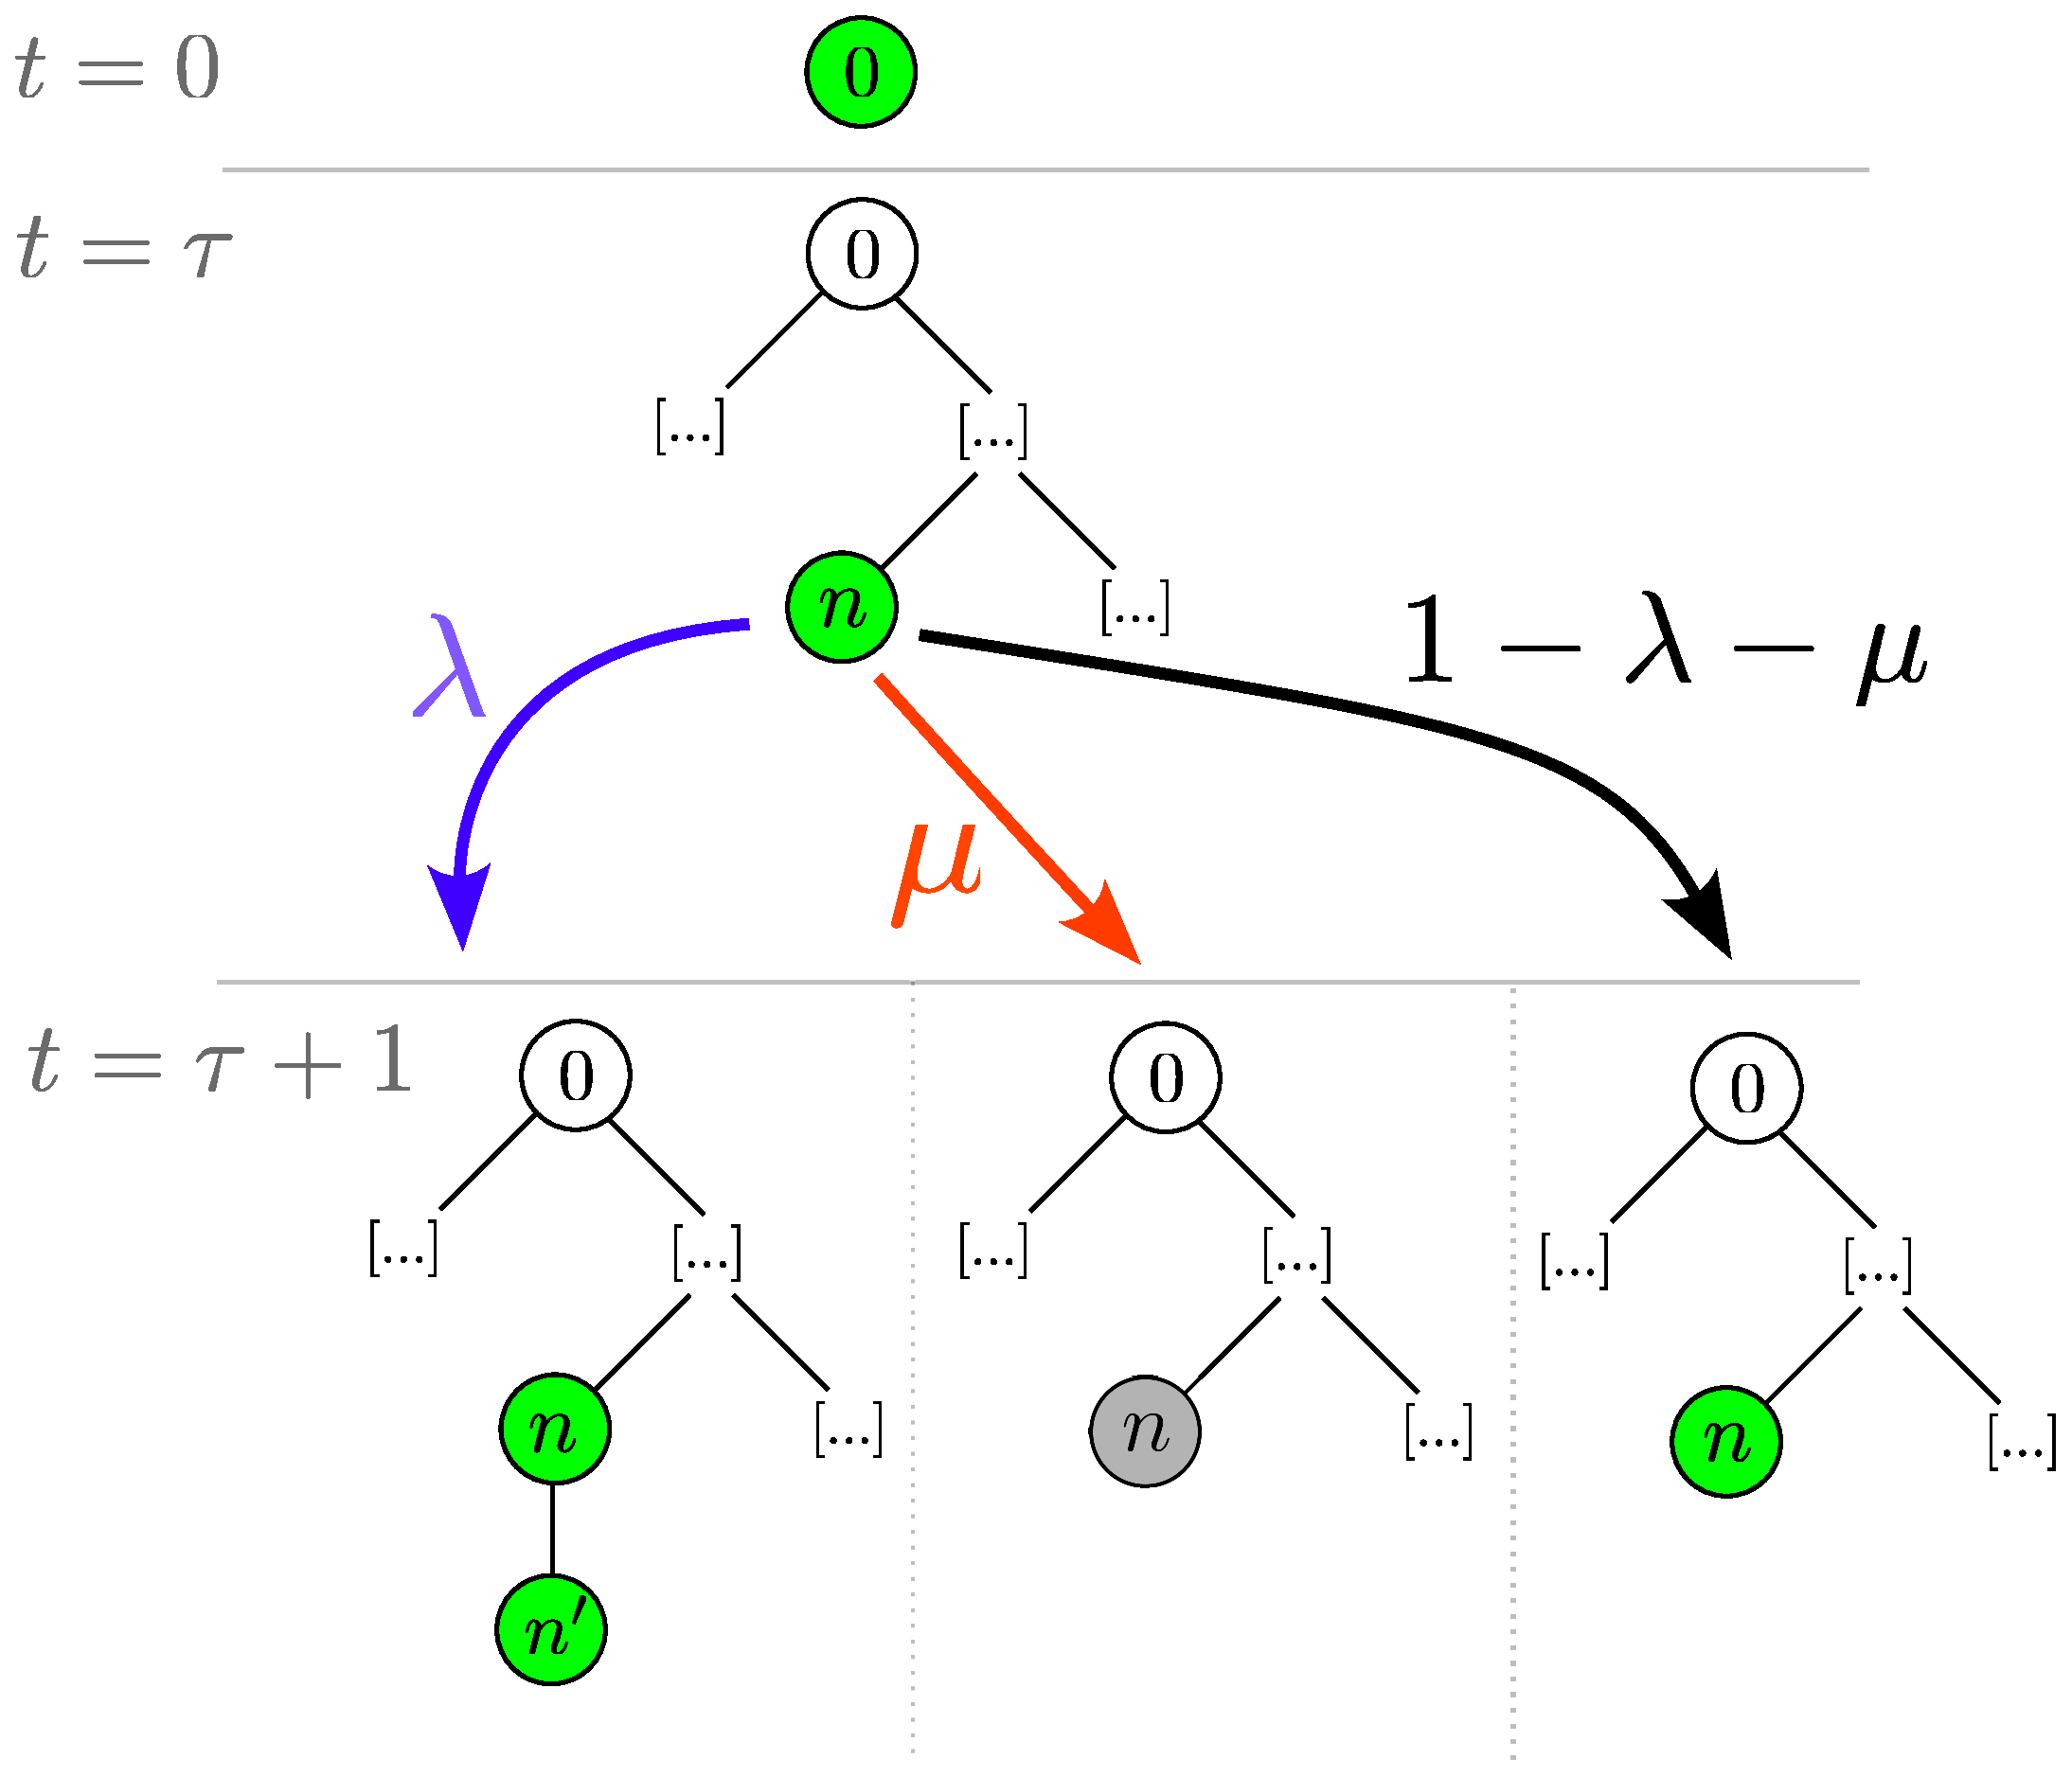
\includegraphics[width=0.7\textwidth]{figures/bd_dynamics.eps}
\caption{\textbf{Example of dynamics for a single simulated tradition} (which appears, with probability $\Lambda$ per unit time, with a single root manuscript). Here, the tradition starts at $t = 0$ with a single root. At $t = \tau$, each living agent (node) has a probability $\lambda$ of giving birth to a new agent, a probability $\mu$ of dying, and a probability $1 - \lambda - \mu$ that nothing happens.}
\label{fig:bd_dynamics}
\end{figure}

This model has proved to be a relevant null hypothesis for the diffusion of manuscripts texts, able in particular to capture most salient topological properties of empirical stemmata~\cite{camps2025transmissiontextswrittencultures}. It however is plagued with major discrepancies with respect to empirical data, most prominently by predicting an exponentially increasing distribution of the production of new witnesses in time (\autoref{fig:intro:distribs}), as well as an exponentially increasing distribution of the population of surviving witnesses in time, as long as the birth rate is superior to the death rate ($\lambda>\mu$).
In order to find a better fitting model, various mechanisms may be added on top of the bare BD process described above to account for known features of historical manuscript traditions.

\begin{figure}[htb]
\centering
\includegraphics[width=0.8\textwidth]{figures/data_cdg.png}
\caption{Time distribution of the \textbf{production} of \emph{i)} new works in the database of Old French chivalric narratives considered in~\cite{camps2025transmissiontextswrittencultures} (solid red) \emph{ii)} new manuscript witnesses in the same corpus (solid black)
\emph{iii)} new witnesses as predicted by a constant-rate Birth-Death model (cr-BD) running over the same period for the same amount of final manuscript (dashed). With the cr-BD, the production of new witnesses per unit time ($\lambda\overline{n}$, where $\lambda$ is the birth rate of the process and $\overline{n}$ the total number of manuscripts already existing at this time) increases exponentially}
\label{fig:intro:distribs}
\end{figure}

\subsection{Modelling text transmission across time, and the need for different classes of manuscripts}

A generalisation that may be applied to any kind of model is the time-variation of its parameters to account for historical factors, whether extrinsic to the dynamics of a specific literary corpus, pertaining to the material conditions of manuscript production or loss, or semi-extrinsic ones such as the popularity of a given literary genre over time. For Classical Greek and Latin traditions, this approach has actually already been attempted by Weitzman~\cite{weitzman_evolution_1987}.

In the case of the the simple Birth-Death model presented above, the expectation value of the number of works (denoted by $\overline{N}(t)$) and living manuscripts ($\overline{n}(t)$) in the population at time $t$ satisfy the following differential equations:
\begin{align}
\frac{\mathrm{d} \overline{n}}{\mathrm{d} t} & = \lambda(t) \overline{n} - \mu(t) \overline{n} + \Lambda\\
\frac{\mathrm{d} \overline{N}}{\mathrm{d} t} & = \Lambda - \mu(t) f_1(t)\label{eq:BDworks}
\end{align}
where $f_1$ represents the number of works manifested by a single living manuscript.\footnote{
An explicit expression for the variation of $f_1$ can be given, making this system closed.
} In particular, the number of manuscript produced per unit time at a given moments writes $\lambda(t) \overline{n}(t) + \Lambda$ (while for the production of works, it is simply $\Lambda$).

The number of surviving witnesses from a given period of time is but a fraction of the total production, due to cumulated losses from this period onward.
From the average total living populations, one can thus compute the density of produced witnesses and works that survived up to some final time $T_f$:
\begin{align}
\rho_n^\text{S}(t) & = \lambda(t) \nbar(t) \mathrm{e}^{- \int_t^{T_f}\mu(\tau) \rmd \tau} \label{eq:nbar_s}\\
\rho_N^\text{S}(t) & = \Lambda \bigg( 1 - P_0(T_f - t | \lambda, \mu) \bigg) \label{eq:Ns_bd}
\end{align}
Where $P_0(\tau| \lambda, \mu)$ is the probability that a tradition consisting of a single witness at time $t=0$ is extinct at time $\tau$ given the history of $\lambda(t)$ and $\mu(t)$ over this period of time (see \autoref{appdx:first}).
Thus, the time-density of surviving manuscripts among those produced at a given time is obtained as the product of the theoretical production rate of manuscripts $\lambda(t) \nbar(t)$ at this time, modulated by a decay factor accounting for posterior losses.

If one would like to fit this abstract model to a given set of data, for any given historical collection of (dated and datable) texts and manuscripts, they would be faced with several difficulties:
\begin{enumerate}
\item the intuition that the time distribution of surviving texts and manuscripts is in itself a good proxy for the time distribution of the total production (preserved and lost), is misleading. Indeed, cumulative losses affect differently older and more recent texts and manuscripts.
\item In the BD model, the contribution of losses is the dominant factor in the time distribution of the production of witnesses, i.e.,  only a tiny fraction of older manuscripts would be able to survive, which is inconsistent with historical data (without assuming levels of production beyond anything reasonable for older periods).
\end{enumerate}
This necessitates the addition to the model of a new element, that can account for the time distributions observed in real datasets.

Indeed, let's consider first the likely misleading intuition that there is a proportionality between the time distribution of surviving manuscripts and the time distribution of the true total population (i.e. including those that were lost afterwards). In other words, the more (the fewer) manuscripts are preserved from a given period, the higher (the lower) the total original production would have been. If we follow this assumption,
it then becomes possible to fit the rates $(\Lambda,\lambda,\mu)$ in time by using empirical data, such as the one that exists for Medieval French literature~\cite{Jonas}.
It is actually on the basis of this assumption (and with the further confrontation to existing expertise about the underlying historic context) that Weitzman determined the variable rates he used to model the transmission of the Greek and Latin classics between 450 BC and AD 1950~\cite{weitzman_evolution_1987}.

Yet, in the context of the BD process envisioned here, this assumption is false. Due to the exponential character of this decay as a function of age $\tau$, the general shape of the time distribution of witnesses creation should be dominated by the contribution of losses rather than reflect significant variations in the production of manuscripts. In other words, the surviving manuscripts would be mostly constituted of fairly recent books, produced at the end of the chronological range. Conversely, there should be only a tiny fraction of older manuscripts able to survive.
This is however inconsistent with empirical data, as can be seen from the case of Old French chivalric narratives (\autoref{fig:intro:distribs})~\cite{camps2025transmissiontextswrittencultures}. Indeed, assuming that the surviving population from  a given time is at any time proportional to the historically produced amount of manuscripts, \emph{i.e.} that $\rho_n^\text{S}(t) = \lambda(t) \nbar(t)$, one can get a first estimate of the values of rates $\Lambda$, $\lambda$ and $\mu$ over time by fitting them to real world chronological data.
This assumption is of course grossly inaccurate, but reintroducing now the decay factor in equation (\ref{eq:nbar_s}) with $\mu(\tau)$ inferred from the first fit, one obtains an estimate of the loss rate distribution over time under a safe lower bound assumption for the amount of manuscript losses. For instance, a manuscript produced in the the year 1450 would be 15 times more likely to survive than one produced in 1300. However, in our case study the observed relative maximum of witness production at the turn of the 14th century would imply significantly higher reproduction rates than what is likely according to historical knowledge of the process of manuscript copying, with most manuscripts being reproduced several times a year.

Thus, a realistic model of text transmission should mitigate the effect of losses to allow the time distribution of surviving witnesses to match more closely the actual history of manuscript and text populations.

\subsection{Not all manuscript are created equal: a two agent-class model} \label{sec:2class_model}

The quality of manuscripts produced during the Middle Ages displays high variability, from low-end, non-ornamented copies to richly illuminated codices. This difference in material qualities often reflects a difference in purpose and fate. While low quality copies are much more likely to be destroyed than higher quality ones, the latter are also less likely to be copied, being kept away from the production circuit as object of use or prestige. In the context of Medieval French epics, this difference takes the form of a distinction, formulated in the 19th century by L.~Gautier, between the so-called ``\textit{manuscrits de librairie}'' (library manuscripts) and ``\textit{manuscrits de jongleurs}'' (jugglers' manuscripts)~\cite{gautier_epopees_1878} (\autoref{fig:manuscript_types}). The ``manuscrits de librairie'', that actually constitute a large majority of the surviving artefacts, are ``well-crafted volumes, even luxurious volumes, where the page is divided into two or three columns, and the text is enhanced with initials, ornate initials, illuminations and
vignettes (…) obviously produced in workshops'' to match the demand of fortunate readers~\cite{tyssens_tradition_1988}. On the other hand, a small number of surviving documents are small-format plain books, often copied with less care on lower quality pieces of parchment~\cite{tyssens_tradition_1988,careri_manuscrits_2006}. If we do not longer believe, as Gautier did, that they were copies made for jugglers, to guide them in their performance, it is quite obvious that ``for once, texts themselves are given more importance than books''~\cite{careri_manuscrits_2006}.

\begin{figure}
\centering
\includegraphics[width=0.25\textwidth]{figures/Bodleian-Library-MS-Digby-23-Part-2_00013_7r.jpg}
\includegraphics[width=0.22\textwidth]{figures/Reg.lat.1616_0237_fa_0117r_m.jpg}

\includegraphics[width=0.7\textwidth]{figures/fr_774.jpg}
\includegraphics[width=0.7\textwidth]{figures/fr_1449.jpg}
\caption{
\textbf{Booklets (top) versus ``library manuscripts'' (middle, bottom)}. A copy of the \textit{Chanson de Roland}, made in England around 1130 (Oxford, Bodleian Library, Digby 23, Part 2, fol. 7r);
a copy of the \textit{Chanson d'Otinel}, made in Saint-Brieuc in 1317 (Vatican, Biblioteca Apostolica Vaticana, Reg. lat. 1616, fol.~117r).
Two manuscripts of the cycle of Guillaume d'Orange, originating from the same Île-de-France workshop in the second half of the 13th century (Paris, Bibliothèque nationale de France, français, 774, fol. 9v-10r; Paris, Bibliothèque nationale de France, français 1449, fol. 9v-10r.
Source: \textit{Gallica}).
}
\label{fig:manuscript_types}
\end{figure}

At the most elementary level, one can account for this heterogeneity of manuscript status by considering a Birth-Death model with two classes of agents featuring different values of their dynamical parameters:
\begin{itemize}
\item
\emph{Diffusion} manuscripts presenting comparatively large values of their reproduction ($\lambda_d$) and death ($\mu_d$) rates.
\item
\emph{Conservation} manuscripts with low values of their respective reproduction and death rates $\lambda_c$ and $\mu_c$.
\end{itemize}
The dynamic of the model is also characterized by an additional parameter $\phi$: for each copy event (happening with rates $\lambda_d$ or $\lambda_c$), the resulting agent produced belongs to the class of conservation manuscript with probability $\phi$, and to the class of diffusion manuscripts with probability $(1 - \phi)$.

Denoting by $\nbar_d$ and $\nbar_c$ the populations of diffusion and conservation manuscripts respectively, their evolution writes
\begin{align}
\frac{\rmd \nbar_d}{\rmd t} & = (1-\phi) (\lambda_d \nbar_d + \lambda_c \nbar_c) - \mu_d \nbar_d\\
\frac{\rmd \nbar_c}{\rmd t} & = \phi (\lambda_d \nbar_d + \lambda_c \nbar_c) - \mu_c \nbar_c
\end{align}
In the limit case $\lambda_c = \mu_c = 0$, the population of surviving conservation manuscripts over time is simply proportional with factor $\phi$ to the living population of diffusion manuscripts $\nbar_d(t)$ at any given time. More generally, for $\lambda_c \ll \lambda_d$ and $\mu_c \ll \mu_d$ , the dynamics of conservation manuscripts is much slower than that of diffusion manuscripts, and keeps record of the instantaneous populations on a longer time scale, so that this models satisfies the requirement identified above, that the extant population should be more representative of the evolution of actual historical population.

\section{Results}

As a first experiment, we present here results obtained by fitting this general model to data for Medieval French texts and witnesses~\cite{Jonas}. Since, for now, we do not have sufficient data on the status of surviving witnesses, i.e. whether they belong to the conservation or diffusion class, we can try a first fit on the limit case, where $\lambda_c = \mu_c = 0$, and the population of surviving conservation manuscripts over time is simply proportional with a constant factor $\phi$ to the living population of diffusion manuscripts $\nbar_d(t)$ at any given time. In this case, it becomes possible to fit the model in proportion to the observed time distribution of surviving witnesses in historical data, that are for now all supposed to be conservation manuscripts (\autoref{fig:bd_time_fit}).

\begin{figure}
\centering
\includegraphics[width=0.8\textwidth]{figures/time_fit_jonas.png}
\caption{\textbf{Number of texts
and conservation manuscripts
produced per year as a function of time}. Solid lines are data obtained from the \emph{Jonas} database of French Medieval texts~\cite{Jonas}. Dashed lines represent the best fit estimate of the expectations values of the corresponding populations under a Birth-Death model with time-varying dynamical parameters, and two classes of agents. Specifically, the dashed lines correspond to the specific case where $\lambda_c = \mu_c = 0$ and $\phi$ is constant over time.
The corresponding values of the parameters for the birth rates of texts ($\Lambda$) and diffusion manuscripts ($\lambda_d$), as well as for the death rate of diffusion manuscripts ($\mu_d$), inferred from least-square interpolation, are also plotted.}
\label{fig:bd_time_fit}
\end{figure}

Of course, this is only a first approach, relatively similar in practice to assuming that the living population is at any time proportional to the surviving population. Further work should try to estimate $\phi$, and its time variation, using historical data, as well as explore different values of $\lambda_c$ and $\mu_c$.

\section{Discussion}

As it has just been shown above, in order to realistically model the evolution of medieval manuscript traditions, the heterogeneity of manuscript survival probabilities, and thus of their material qualities, have to be accounted for.

The model that we outline in section \ref{sec:2class_model} is a first elementary step in that direction. Building incrementally over the simple Birth-Death model which has been so far the baseline of quantitative modelling of manuscript traditions, we introduce a heterogeneity of dynamical parameters across the population of manuscripts by considering two classes of agents. While this is a gross oversimplification of reality, as the material characteristics of written artefacts vary continuously over a wide range of qualitative parameters, one expects the emergent behaviour observed --~namely the increased evenness of the time distributions of surviving manuscripts~-- to be robust under further generalisation.

An extreme case of the model that we propose allows to assume that surviving populations of texts and witnesses are representative of actual historical populations, yielding approximate estimates of the variation of production rates over time. Indeed, the first results (\autoref{fig:bd_time_fit}) displays some qualitative dynamics, such as the increase of manuscript production during the second half of the 12th century and the 13th century, or the crisis of the 14th century. These dynamics are more sensible from an historical perspective than a steady exponential increase of production, as seen in the previous constant rate BD model.

Yet, this remains an oversimplification that needs to be mitigated by more careful parameter estimates. Indeed, the introduction of a new degree of freedom into the Birth-Death dynamics comes at the cost of additional free parameters $\phi$, $\lambda_c$ and $\mu_c$. While the internal dynamics of the class of so-called \emph{conservation manuscripts}, ruled by parameters $(\lambda_c, \mu_c)$ is assumed to be dominated by (much reduced) losses, further comparison of the model to empirical data will require estimations of the production ratio $\phi$ between conservation and \emph{diffusion} copies, that may be itself subject to wide variations in time.

Such estimations may rely on the exploitation of additional data, including statistics on codicological features, as well as topological properties of the stemmata of known textual traditions, in the line of previous works on the constant rate Birth-Death model. In particular, this model could be a partial explanation to the high degree of bifidity and imbalance observed on stemmata~\cite{camps2025transmissiontextswrittencultures}, by accounting for the survival of high-branching, less populated branches of manuscript traditions. Finally, further work should investigate the effects of this new model on the distribution of witnesses per text.

\section*{Code and material availability}

Data and code implementing the models described here is available on Zenodo,\\ doi:\href{https://doi.org/10.5281/zenodo.17467625}{10.5281/zenodo.17467625}.

\section*{Acknowledgements}

\includegraphics[width=0.15\textwidth, trim={1cm 7cm 1cm 0cm}, clip]{figures/LOGO_ERC-FLAG_EU_(1).jpg}
Funded by the European Union (ERC, LostMA, 101117408). Views and opinions expressed are however those of the author(s) only and do not necessarily reflect those of the European Union or the
European Research Council. Neither the European Union nor the granting authority can be held responsible for them.

This work has received support under the Major Research Program of PSL Research University ``CultureLab'' launched by PSL Research University and implemented by ANR with the references ANR-10-IDEX-0001.

\printbibliography

\appendix

\section{Population statistics in Birth-Death model with variable rates} \label{appdx:first}

In order to derive the loss term in equation (\ref{eq:BDworks}) for the evolution of the population of texts under the Birth-Death process considered in this paper, one needs to perform a more careful accounting of the internal statistical structure of the populations of manuscripts (agents) and texts (trees).

Considering a population generated by the Birth-Death model, we denote by $p_k(t)$ for $k \geq 1$ the probability that a text consisting initially of one manuscript is manifested by exactly $k$ extant manuscript at time $t$ or, put in another way, the frequency class of independent trees in the population consisting of $k$ living agents. While new independent traditions consisting of a single living original manuscript are constantly generated at rate $\Lambda$, the class traditions consisting of $k$ witnesses may, during an elementary time step $[t, t+\rmd t]$
\begin{itemize}
\item
Gain a text from internal birth event occurring in some tradition consisting of $k-1$ witnesses, with probability $\lambda(t) (k-1) \rmd t$ per corresponding traditions;
\item
Gain a text from a death event occurring in some tradition consisting of $k+1$ witnesses, with probability $\mu(t) (k+1) \rmd t$ per corresponding traditions;
\item
Lose or gain a text by a death or birth event occurring within a tradition the class $f_k$, with probability $(\lambda(t) + \mu(t)) \rmd t$ per works in the class.
\end{itemize}
Thus the time evolution of the quantities $\{p_k(t)\}_{k \geq 1}$ writes
\begin{align}
\frac{\rmd p_1}{\rmd t} & = 2 \mu(t) p_2 - (\mu(t) + \lambda(t)) p_1\\
\frac{\rmd p_k}{\rmd t} & = \lambda(t) (k-1) p_{k-1} + \mu(t) (k+1) p_{k+1} - (\mu(t) + \lambda(t)) k p_k~~~~\text{for}~~~~k \geq 2
\end{align}
With the probability of extinction of manuscripts being simply
\begin{align}
\frac{\rmd p_0}{\rmd t} = \mu(t) p_1
\end{align}
This system of linear differential equations can be explicitly solved, thus yielding an expression for the loss rate in (\ref{eq:BDworks}): solving this equation for $\Lambda = 0$, with $p_1(0) = 1$ and $p_k(0) = 0$ otherwise, one can evaluate the probability of extinction appearing in equation (\ref{eq:Ns_bd}) as:
\begin{align}
P_0(\tau | \lambda, \mu) = f_0(\tau)
\end{align}
while the average number of works manifested at time $t$ by a single witness writes
\begin{align}
f_1(t) = \int_{0}^t \Lambda(\tau) p_0(t-\tau) \mathrm{d} \tau
\end{align}
\end{document}